\documentclass[a4paper,12pt]{article}

\usepackage{graphicx}
\usepackage{amsmath}
\usepackage{array}
\usepackage{booktabs}
\usepackage{hyperref}
\usepackage{float}
\title{\textbf{Scientific Calculator using Arduino}}
\author{Arnav Yadnopavit\\EE24BTECH11007}
\date{\today}

\begin{document}

\maketitle
\newpage
\tableofcontents

\newpage

\section{Introduction}
A scientific calculator is an essential tool for performing complex mathematical operations such as trigonometry, logarithms, exponentiation, and numerical methods. This project implements a scientific calculator using an Arduino board, a 16x2 LCD display, and a button matrix. The calculator is designed to evaluate expressions efficiently and accurately using numerical methods like the **CORDIC algorithm** for trigonometric functions and the **Runge-Kutta 4th order method (RK4)** for logarithms and exponentiation.

\section{Components}
This section briefly describes the components used in the project.

\subsection{Arduino Board}
The Arduino acts as the central processing unit, handling input from the button matrix, performing calculations, and displaying results on the LCD.

\subsection{16x2 LCD Display}
The 16x2 LCD display is used to show the input expression and the computed result. It operates in 4-bit mode to save I/O pins.

\subsection{Button Matrix}
A **4x5 button matrix** is used for input. It operates in two modes:
\begin{itemize}
    \item \textbf{Normal Mode}: Directly enters numbers and basic operations.
    \item \textbf{Shift Mode}: Activates advanced functions like trigonometry and logarithms.
\end{itemize}

\subsection{Push Button for Shift Mode}
A dedicated shift button enables alternate functions for each key.

\subsection{Resistors and Wires}
Resistors ensure proper signal transmission, while jumper wires connect the components.
\begin{table}[H]
    \centering
    \renewcommand{\arraystretch}{1.2} % Adjust row height
    \begin{tabular}{|c|c|}
        \hline
        \textbf{Component} & \textbf{Arduino Pin} \\
        \hline
        \multicolumn{2}{|c|}{\textbf{Button Matrix}} \\
        \hline
        Row 1 & 2 \\
        Row 2 & 3 \\
        Row 3 & 4 \\
        Row 4 & 5 \\
        Column 1 & 6 \\
        Column 2 & 7 \\
        Column 3 & 8 \\
        Column 4 & 9 \\
        Column 5 & 10 \\
        \hline
        \multicolumn{2}{|c|}{\textbf{Shift Button}} \\
        \hline
        Shift Button & 13 \\
        GND & GND \\
        \hline
        \multicolumn{2}{|c|}{\textbf{LCD Display (16x2, Non-I2C)}} \\
        \hline
        LCD RS & A0 \\
        LCD EN & A1 \\
        LCD D4 & A2 \\
        LCD D5 & A3 \\
        LCD D6 & A4 \\
        LCD D7 & A5 \\
        \hline
    \end{tabular}
    \caption{Circuit Connections of the Scientific Calculator}
    \label{tab:circuit_connections}
\end{table}
\newpage

\begin{figure}[H]
    \centering
    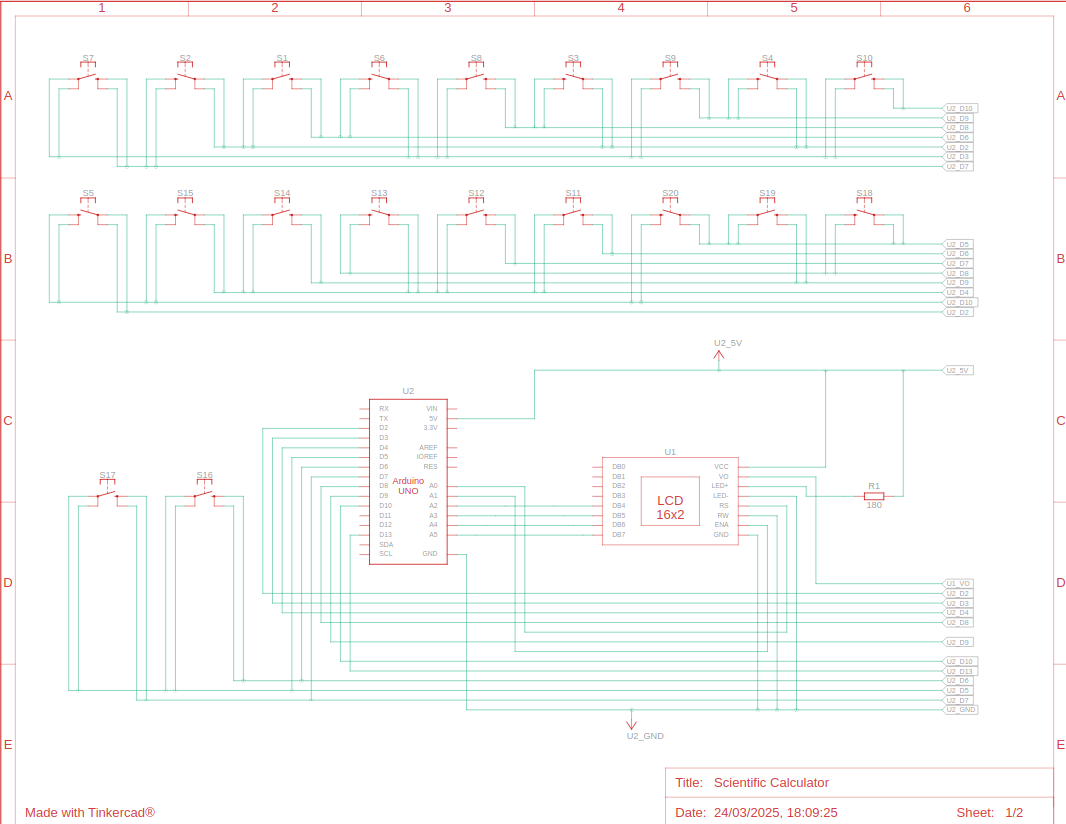
\includegraphics[width=\textwidth]{figs/circuit1.png}
    \caption{Circuit Diagram of the Scientific Calculator (Sheet 1)}
    \label{fig:circuit1}
\end{figure}

\begin{figure}[H]
    \centering
    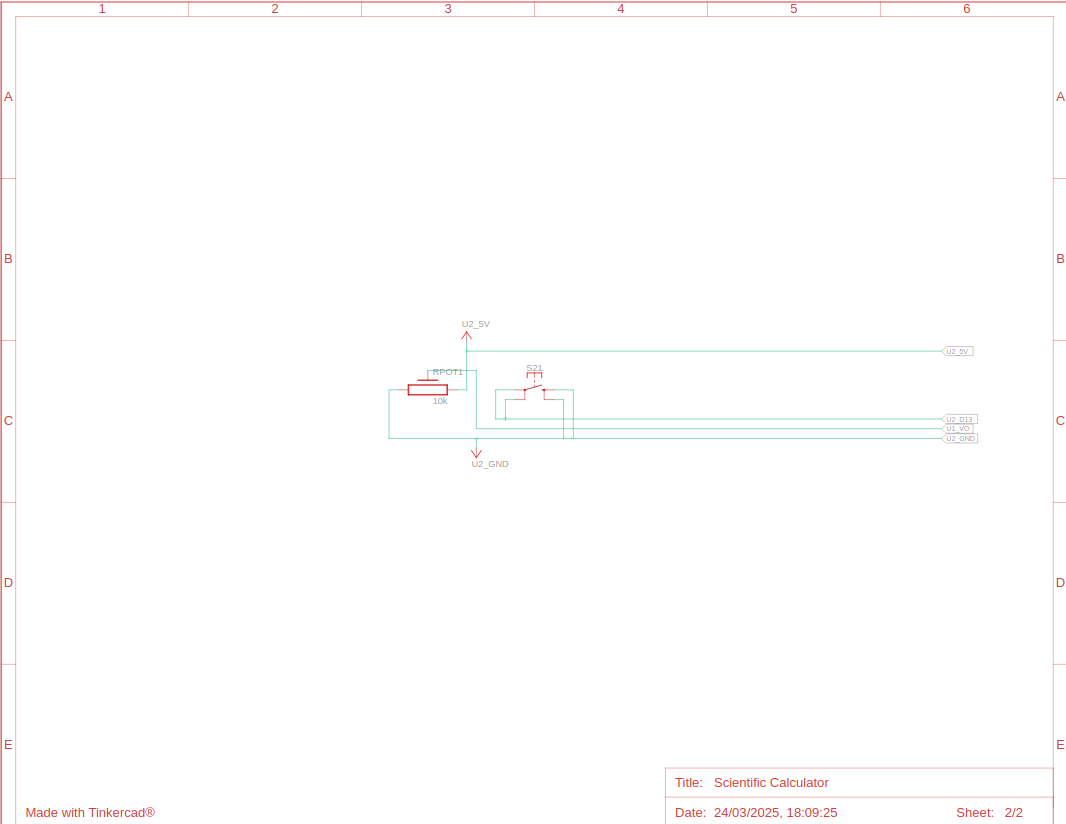
\includegraphics[width=\textwidth]{figs/circuit2.png}
    \caption{Circuit Diagram of the Scientific Calculator (Sheet 2)}
    \label{fig:circuit2}
\end{figure}

\section{Functions Available}
The calculator supports a variety of mathematical operations.

\subsection{Normal Mode Button Layout}
\begin{table}[h]
    \centering
    \begin{tabular}{|c|c|c|c|c|}
        \hline
        1 & 2 & 3 & / & C \\
        \hline
        4 & 5 & 6 & * & D \\
        \hline
        7 & 8 & 9 & - & ( \\
        \hline
        . & 0 & = & + & ) \\
        \hline
    \end{tabular}
    \caption{Normal mode button layout}
    \label{tab:normal_buttons}
\end{table}

\subsection{Shift Mode Button Layout}
\begin{table}[h]
    \centering
    \begin{tabular}{|c|c|c|c|c|}
        \hline
        $\sin$ & $\cos$ & $\tan$ & $x^y$ & C \\
        \hline
        ! & $\pi$ & $e$ & $|x|$ & D \\
        \hline
        log & ln & sqrt & cbrt & r \\
        \hline
        $sin^{-1}$ & $cos^{-1}$ & $tan^{-1}$ & $x^2$ & $x^3$ \\
        \hline
    \end{tabular}
    \caption{Shift mode button layout}
    \label{tab:shift_buttons}
\end{table}

\newpage

\section{Numerical Methods}
To ensure accuracy in mathematical computations, this calculator uses two powerful numerical methods: CORDIC for trigonometric functions and RK4 for logarithmic and exponential functions.

\subsection{CORDIC Algorithm for Trigonometric Functions}
CORDIC (COordinate Rotation DIgital Computer) is an iterative algorithm used for computing trigonometric functions efficiently without floating-point operations.

\subsubsection{CORDIC Equations}
\[
x_{i+1} = x_i - d_i \cdot y_i \cdot 2^{-i}
\]
\[
y_{i+1} = y_i + d_i \cdot x_i \cdot 2^{-i}
\]
\[
z_{i+1} = z_i - d_i \cdot \text{atan}(2^{-i})
\]
where:
\begin{itemize}
    \item \( x, y \) represent the coordinates of the rotated vector.
    \item \( z \) is the angle being processed.
    \item \( d_i \) is the sign of \( z \).
\end{itemize}
\subsubsection{Applications in the Calculator}
\begin{itemize}
    \item $\sin(x) , \cos(x), \tan(x)$
\end{itemize}
\subsection{Runge-Kutta 4th Order Method (RK4)}
The RK4 method is a numerical approach for solving differential equations and is used in this calculator for logarithmic and power functions.

\subsubsection{RK4 Equations}
\[
k_1 = h f(x_n, y_n)
\]
\[
k_2 = h f(x_n + \frac{h}{2}, y_n + \frac{k_1}{2})
\]
\[
k_3 = h f(x_n + \frac{h}{2}, y_n + \frac{k_2}{2})
\]
\[
k_4 = h f(x_n + h, y_n + k_3)
\]
\[
y_{n+1} = y_n + \frac{1}{6} (k_1 + 2k_2 + 2k_3 + k_4)
\]

\subsubsection{Applications in the Calculator}
\begin{itemize}
    \item \textbf{Logarithms}: Computing \( \ln(x) \) and \( \log_{10}(x) \).
    \item \textbf{Exponentiation}: Evaluating \( x^n \).
    \item \textbf{Square and Cube Roots}: Computing \( \sqrt{x} \) and \( \sqrt[3]{x} \).
    \item \textbf{Inverse Trigonometric Functions}: \( \sin^{-1}(x) \), \( \cos^{-1}(x) \), and \( \tan^{-1}(x) \).
\end{itemize}


\section{Expression Evaluation Logic}
To handle complex expressions, the calculator uses:
\begin{itemize}
    \item **Stack-based computation**: Uses two stacks for values and operators.
    \item **Operator precedence rules**: Implements precedence to ensure correct order of operations.
    \item **String parsing**: Extracts numbers, operators, and function names.
    \item **Error handling**: Handles division by zero and invalid inputs.
\end{itemize}

\section{Implementation Challenges and Solutions}
\begin{itemize}
    \item **Handling Button Multiplexing**: Since the number of input pins is limited, a multiplexing technique was used to read button presses efficiently.
    \item **Non-I2C LCD Handling**: The LCD was operated in 4-bit mode to optimize pin usage.
    \item **Efficient Mathematical Computation**: Using CORDIC and RK4 improved accuracy while reducing computation time.
\end{itemize}

\section{Conclusion}
This scientific calculator successfully implements a variety of mathematical functions using efficient numerical methods. The combination of CORDIC and RK4 ensures accurate and fast computations. The button matrix provides an intuitive interface, making it a practical and functional scientific calculator.\\
For codes refer\\
\url{https://github.com/ArnavYadnopavit/EE1003/tree/main/Calculator}\\

\centering
Thank you

\end{document}
